\documentclass{beamer}
\usepackage[orientation=portrait,size=a0,scale=1.3,debug]{beamerposter}
\mode<presentation>{\usetheme{me388}}
\usepackage[none]{hyphenat}
\usepackage{mathspec}
\setallmainfonts{Archivo Narrow}
\setsansfont[BoldFont={Archivo Narrow Bold}]{Archivo Narrow}
\setmonofont[BoldFont={Inconsolata}]{Inconsolata}

\newfontfamily\titlefont[BoldFont={Archivo Narrow}]{Archivo Narrow}
\usepackage{hyperref} %enable hyperlink for urls
\usepackage{ragged2e}
\let\raggedright=\RaggedRight
\usepackage[font=small,margin=0pt,labelfont=bf,justification=justified]{caption}
\usepackage{array,booktabs,tabularx}

\newcolumntype{Z}{>{\centering\arraybackslash}X} % centered tabularx columns
%\sisetup{per=frac,fraction=sfrac}

\title{\huge\titlefont{Crystal structure prediction for next-generation battery anodes}}
\author{\titlefont{Matthew Evans\\[1ex]\texttt{me388@cam.ac.uk}}}
\institute{\titlefont{TCM Group, Cavendish Laboratory, University of Cambridge}}

% edit this depending on how tall your header is. We should make this scaling automatic :-/
\newlength{\columnheight}
\setlength{\columnheight}{104cm}

\begin{document}
\begin{frame}
\begin{columns}
	\begin{column}{.65\textwidth}
		\begin{beamercolorbox}[center]{postercolumn}
			\begin{minipage}{.98\textwidth}  % tweaks the width, makes a new \textwidth
				\parbox[t][\columnheight]{\textwidth}{ % must be some better way to set the the height, width and textwidth simultaneously
            \begin{myabstract}{Abstract}
            In this work, we perform \textbf{high-throughput crystal structure prediction} on materials that have great promise as conversion anodes for next-generation Li/Na-ion batteries, namely transition and post-transition metal phosphide alloys. Using \emph{ab initio} random structure searching \cite{Pickard2011} and related methods, previous work on phosphorous anodes \cite{Mayo2016} is extended in an attempt to find \texbf{sustainable materials} with \textbf{manageable volume expansion} during charging.
            \end{myabstract}
            \begin{columns}
	\begin{column}{.48\textwidth}
		\begin{beamercolorbox}[left]{postercolumn}
        \begin{minipage}{\textwidth}  % tweaks the width, makes a new \textwidth
				\parbox[t][\columnheight]{\textwidth}{ % must be some better way to set the the height, width and textwidth simultaneously
              \begin{myblock}{Motivation}
                  In order to displace fossil fuels in the global energy infrastructure, sustainable, high-capacity energy storage solutions are urgently required. Lithium ion batteries have already revolutionised the world, bringing about the advent of portable electronics --- how can we extend this technology to grid applications?
            \begin{figure}
              \centering
              \includegraphics[width=\textwidth]{img/LiPX.png}
              \captionsetup{width=0.9\textwidth}
              \caption{Theoretical capacities of ternary conversion anodes for Li-ion batteries, calculated from known phases, with phosphide materials highlighted. Points are coloured by theoretical volume expansion from delithiated to lithiated states. The red point shows the peak capacities of a graphite anode. Structures from the Open Quantum Materials Database \cite{Kirklin2015}.}
            \end{figure}

              Anodes of commercial Li-ion batteries are made of graphite, with gravimetric capacity limited to 372 mAh/g (LiC$_6$) as Li ions intercalate between the graphite layers. These anodes are limited in rate capability by the sluggishness of the intercalation process --- charging too rapidly leads to Li plating and dangerous shorting of the cell. As an alternative, materials that alloy with Li, e.g. Si or P, can be used to greatly increase capacity by an order of magnitude (2597 mAh/g Li$_3$P). This increased capacity comes at the expense of extreme volume expansion, reducing cyclability and safety.

Conversion anodes are a middle ground: consisting of AB alloys, they can exhibit intercalation, alloying and displacement reactions upon cycling. The elements A and B can be tuned such that one forms high-capacity alloys (e.g. P) and the other acts as an inactive (or less active) buffer matrix that mitigates volume expansion.

					\end{myblock}
					\begin{myblock}{Phosphide conversion anodes}
              An idealised conversion reaction for an X$_x$P$_y$ binary can be described by:
          \[ \text{X}_x \text{P}_y + z\,\text{Li} \to n\,\text{Li}_\delta\text{X}_{x'} + y\,\text{Li}_3\text{P}.\]

          Conversion anodes store Li by converting the original anode material into an Li-rich phase, plus a displaced phase (which may itself contain Li). By mapping out the ternary configuration space, the stable reaction pathways can be enumerated and ranked by thermodynamic and kinetic preferability. Due to the enormity of the space, we focus on sustainable materials \cite{Grey2016}, namely \{Li, Na\}-\{Ti, Cu, Zn, Al, Sn\}-P.
      \end{myblock}\vfill
		}\end{minipage}\end{beamercolorbox}
	\end{column}
    % no idea why this is needed for proper spacing
  \begin{column}{.00\textwidth}
    \end{column}
  \begin{column}{.48\textwidth}
		\begin{beamercolorbox}[right]{postercolumn}
			\begin{minipage}{\textwidth} % tweaks the width, makes a new \textwidth
				\parbox[t][\columnheight]{\textwidth}{ % must be some better way to set the the height, width and textwidth simultaneously
					\begin{myblock}{Crystal structure prediction}
              Broadly, crystal structure prediction is the act of searching for the lowest energy configurations of atoms under different conditions. When modelling batteries, we sample various compositions as if the system were connected to an infinite reservoir of the active ion.
              
              The primary method used here for performing an unbiased sampling across various compositions is \emph{ab initio} random structure searching (AIRSS) \cite{Pickard2011}. By randomly generating many structures with "sensible" symmetries and connectivities and relaxing them with forces from rough density-functional theory (DFT) calculations, the energy landscape can be efficiently mapped. Computing the convex hull of formation energies against elemental (or otherwise) chemical potentials yields the zero-temperature phase diagram of the system.
            \begin{figure}
                \centering
              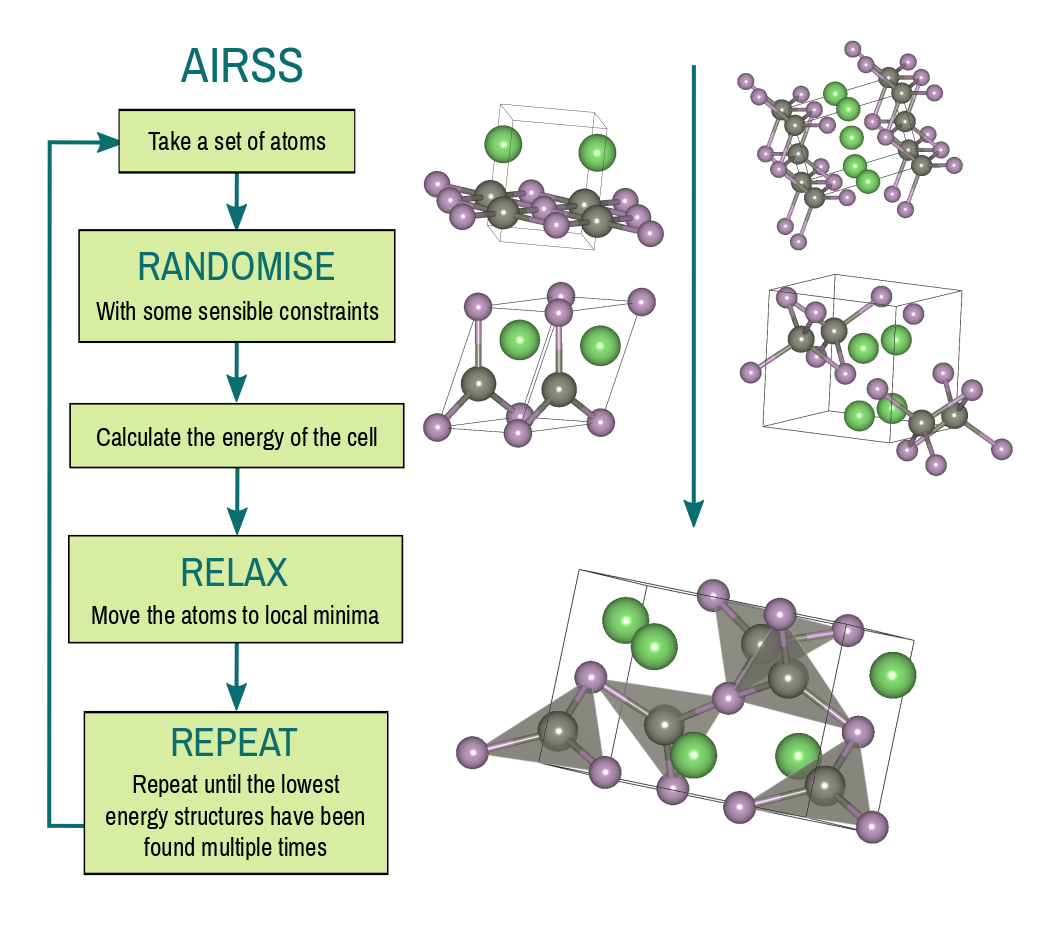
\includegraphics[width=0.9\textwidth]{img/airss.png}
          \end{figure}
              
              With sufficient sampling, AIRSS will find the global minima, however, when the search space is very large, this may require hundreds of thousands of calculations. Exploiting experimental and theoretical databases by swapping atomic types from known crystal structures will often yield undiscovered structures; this can be thought of as an interpolation across all chemistry.
                \vspace{0.2in}
              \begin{figure}
                \centering
              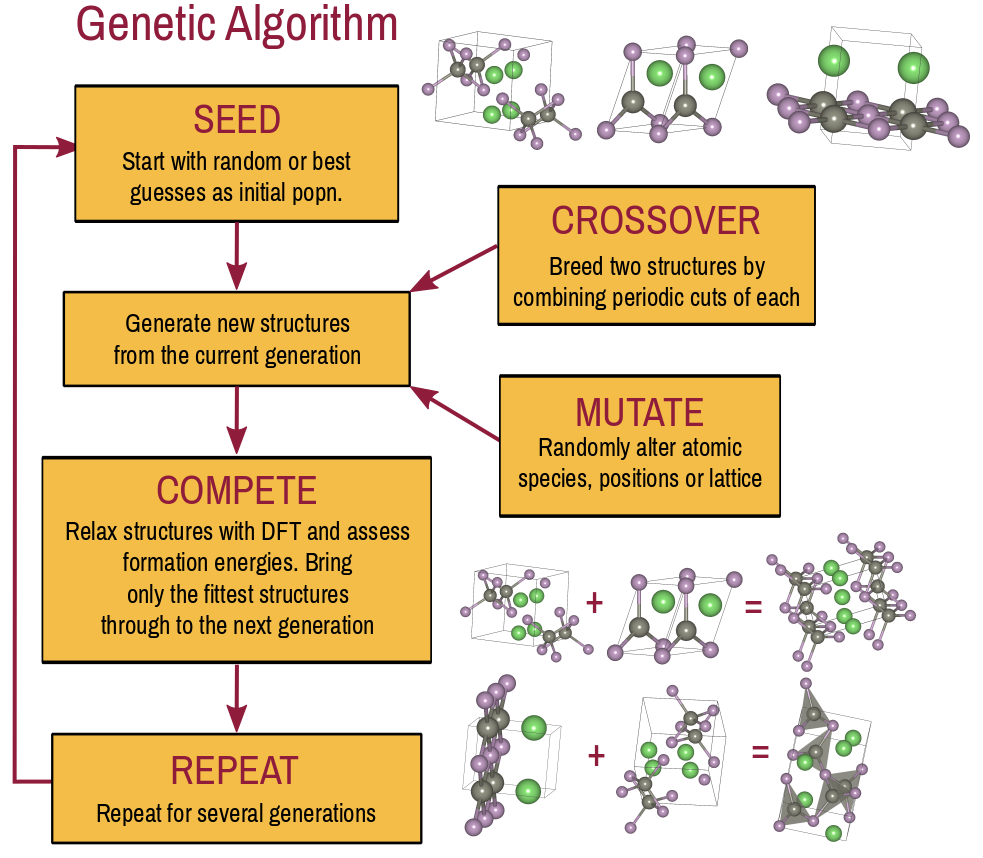
\includegraphics[width=0.9\textwidth]{img/ga.png}
          \end{figure}

An additional approach used here is to extrapolate from the unbiased sampling of AIRSS using a genetic algorithm. Starting from an initial population, structures are randomly mutated and combined, relaxed and then ranked by "fitness" (formation energy) to form the next generation. This is repeated for many generations until no new structures are found (stagnation).

					\end{myblock}\vfill
		}\end{minipage}\end{beamercolorbox}
	\end{column}
  \end{columns}
		}\end{minipage}\end{beamercolorbox}
  \end{column}
    
	\begin{column}{.32\textwidth}
		\begin{beamercolorbox}[center]{postercolumn}
			\begin{minipage}{.98\textwidth} % tweaks the width, makes a new \textwidth
				\parbox[t][\columnheight]{\textwidth}{ % must be some better way to set the the height, width and textwidth simultaneously
            \begin{myblock}{Li-P-Zn}


          An example of interim results for the Li-P-Zn system are shown below, the result of around 10,000 DFT relaxations.

            \begin{figure}
                \centering
              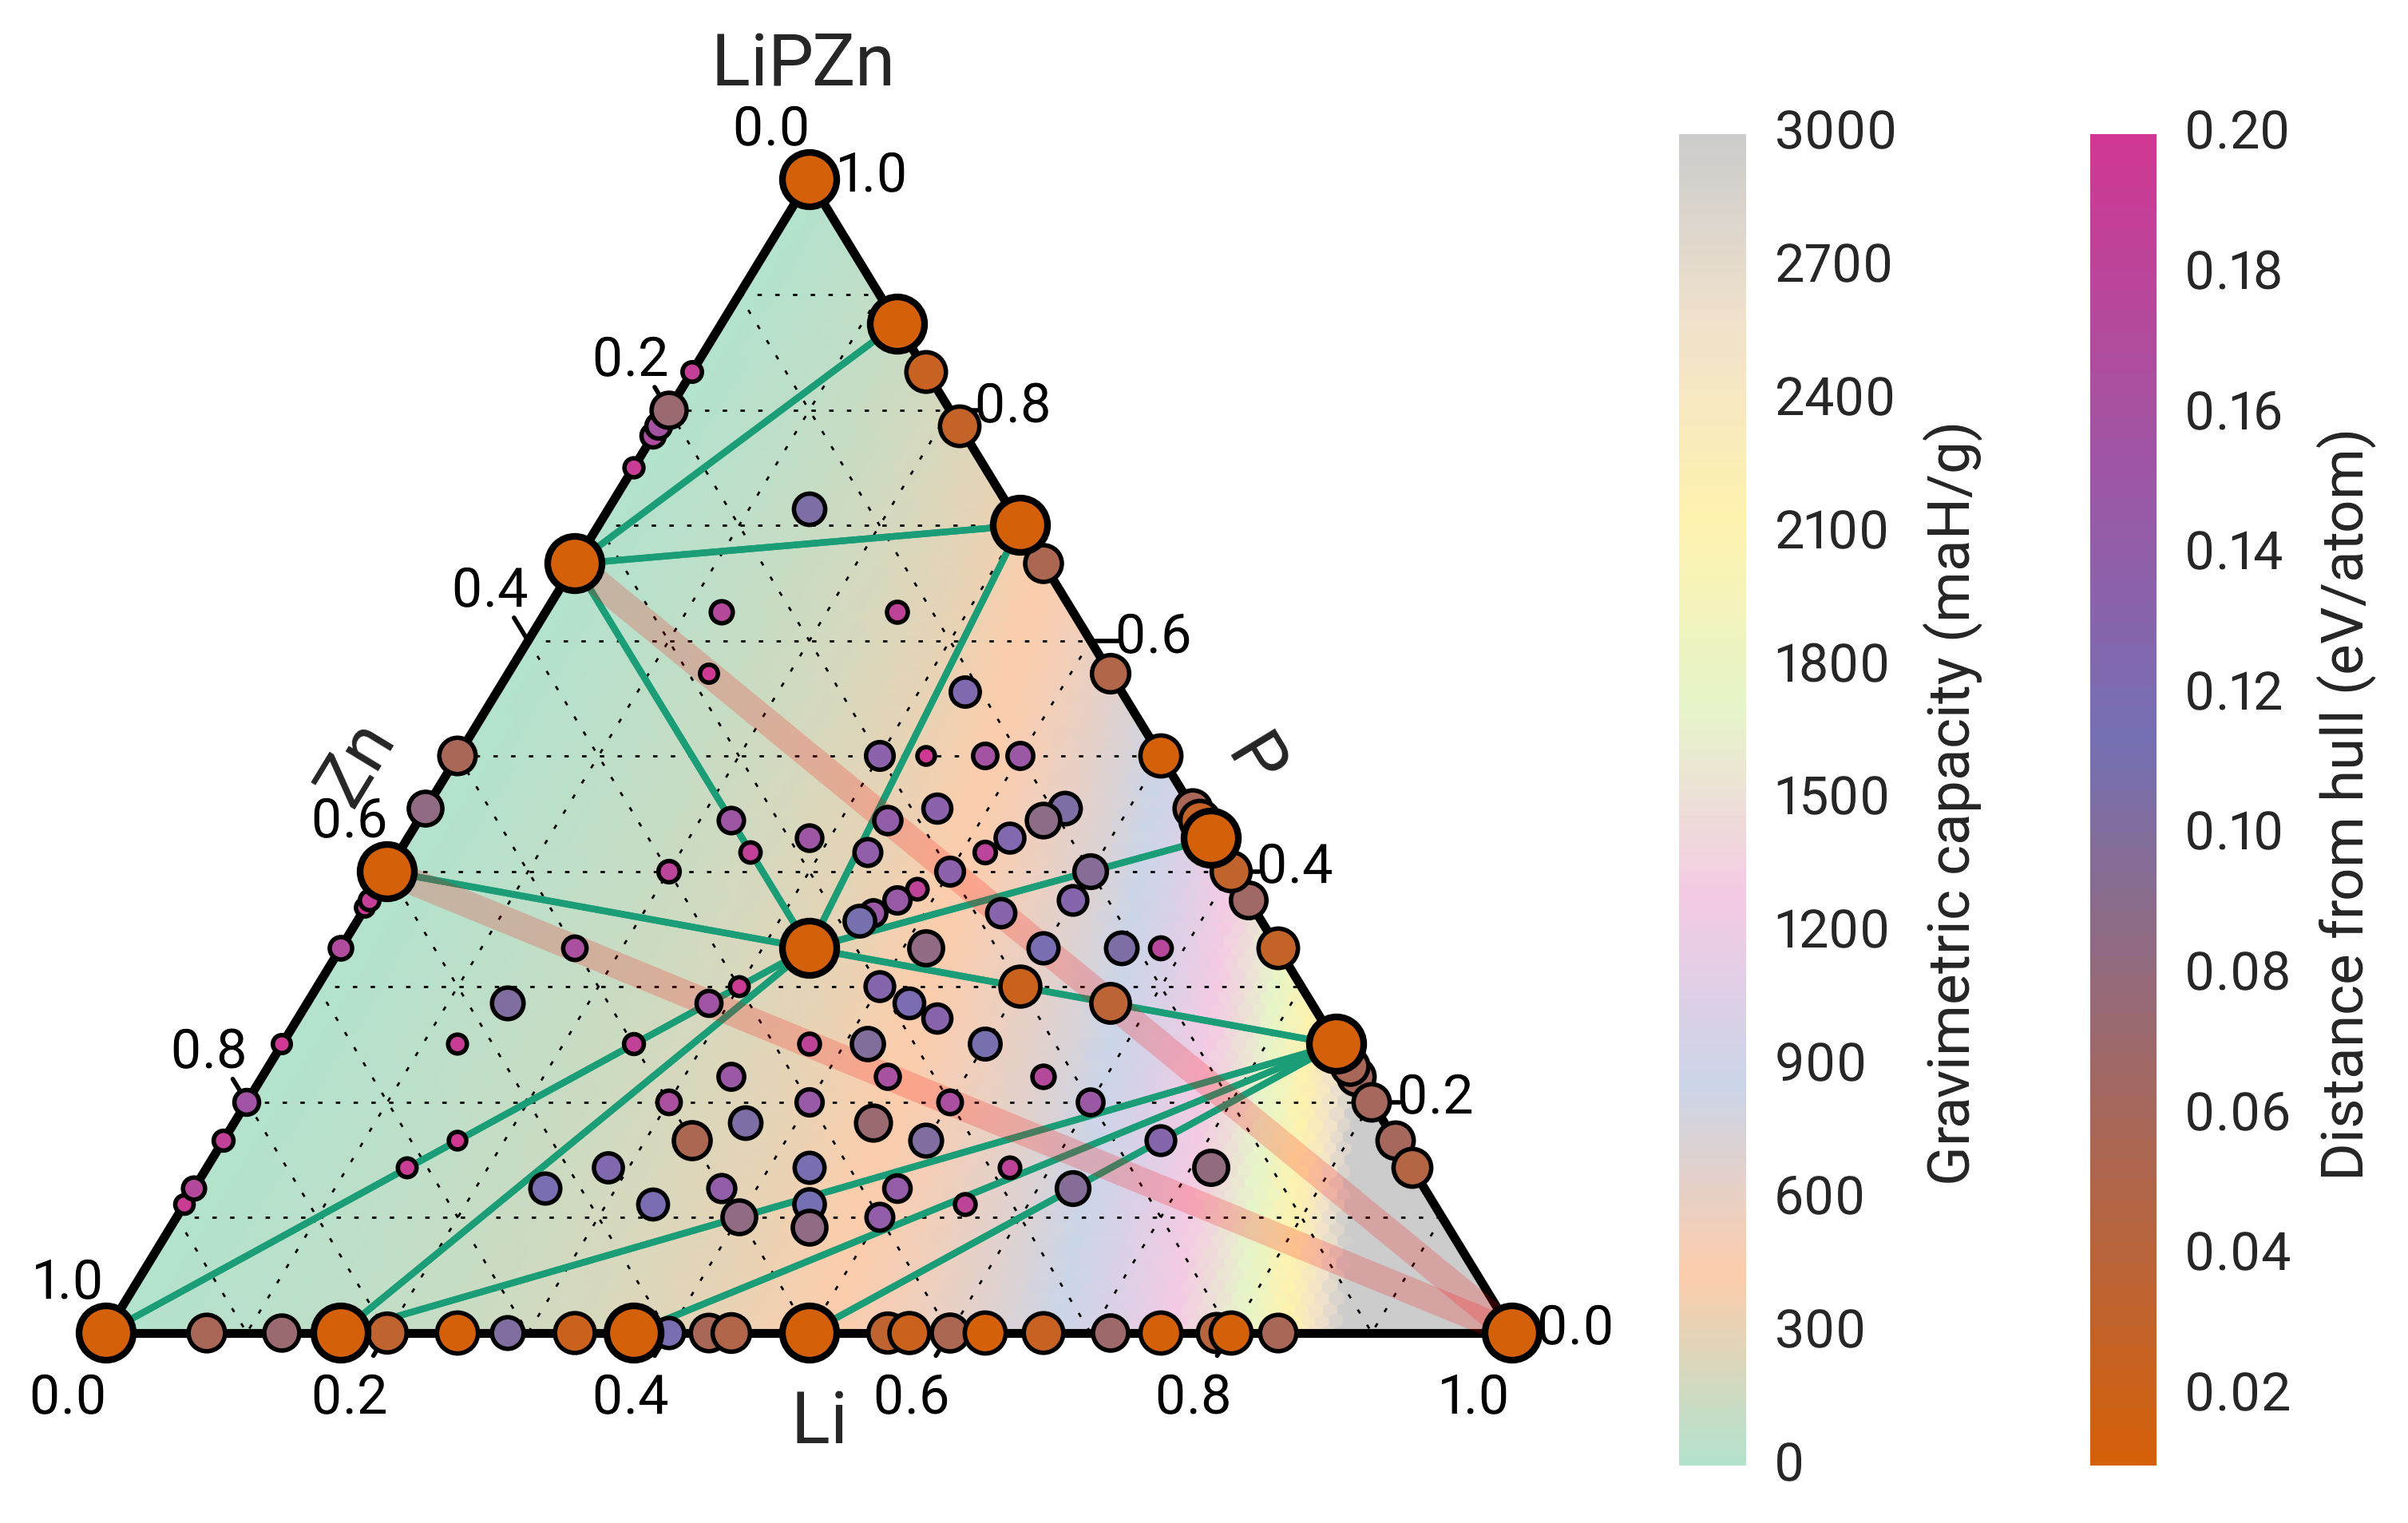
\includegraphics[width=0.9\textwidth]{img/LiPZn.png}
              \captionsetup{width=0.9\textwidth}
              \caption{Ternary phase diagram of the Li-P-Zn system, with points coloured by degree of metastability, and space coloured by gravimetric capacity at that composition.}
            \end{figure}

            The lowest energy structures from the searching stage have been polished to a higher level of accuracy. Voltage curves can then be calculated and compared against experiment. These calculations predict maximum gravimetric capacities of the two known Zn-P alloys as 1473 mAh/g and 934 mAh/g for ZnP$_2$ and Zn$_3$P$_2$ respectively, with manageable volume expansions of 147\% and 122\%. Each phase exhibits an initial voltage around 1 V, suitably high to prevent lithium dendrite formation.

Several novel metastable phases are predicted (e.g Li$_4$P$_2$Zn, Li$_5$P$_3$Zn$_2$) which reaction pathways that dominate, dependent on kinetic effects. Knowledge of these phases allows us to predict the possible voltage curves from each of these pathways for comparison with experiment. By using structural similarity as a proxy for activation barriers, it is hoped that the dominant pathways can be elucidated from first principles.

          \end{myblock}
          \begin{myblock}{Summary \& Outlook}
              \begin{itemize}
                  \item We are performing computational crystal structure prediction across a region of materials space with great promise for sustainable, high-capacity anodes for Li and Na-ions batteries.
                  \item Once each phase diagram is complete, electrochemical and spectroscopic properties can be computed and used in conjunction with experiment to improve our understanding of the mechanisms of battery operation.
                  \item Metastable phases can be included into our model to investigate the effects of finite temperature and crystalline disorder on our predictions.
                  \item The methods presented here can be extended to new the paradigms of K, Al and Mg-ion batteries. These multi-valent ions have abundances on Earth comparable to that of Na and a factor of 10$^3$ greater than that of Li \cite{Grey2016}.
                \end{itemize}
					\end{myblock}\vfill
					\begin{myblock}{References}
						\footnotesize
            \bibliographystyle{unsrt}
						\bibliography{references}
					\end{myblock}\vfill
		}\end{minipage}\end{beamercolorbox}
	\end{column}
\end{columns}
\end{frame}
\end{document}
